\section{Durchführung}
Zu Beginn des Versuchs wird die Zeitkonstante RC bestimmt. Dies erfolgt über die in
Abbildung \ref{fig:RC2} zu sehende Schaltung. Das Oszilloskop wird so eingestellt, dass
ein Entladeforgang der Kondensatorspannung sichtbar wird. Mit Hilfe der
Cursor-Funktion am Oszilloskop werden Messdaten der Kondensatorspannung $U_{C}$ und
der Zeit $t$ erfasst.
\begin{figure}[H]
  \centering
  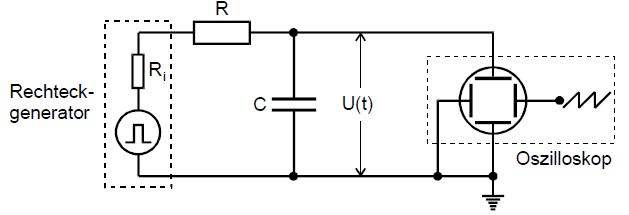
\includegraphics{RC2.JPG}
  \caption[height=5cm]{Messschaltung zur bestimmung der Zeitkonstante.}
  \cite{skript}
  \label{fig:RC2}
\end{figure}
\label{sec:Durchführung}
Anschließend wird die Amplitude $A$ der Kondensatorspannung in Abhängigkeit der
Frequenz gemessen. Dies erfolgt mit derin Abbildung \ref{fig:RC3} dargesellten Schaltung.
\begin{figure}[H]
  \centering
  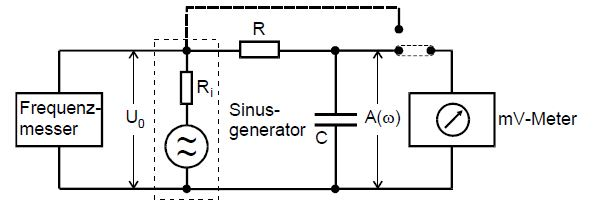
\includegraphics[height=5cm]{RC3.JPG}
  \caption{Messschaltung zur Untersuchung der Frequenzabhängigkeit der Kondensatorspannung.}
  \cite{skript}
  \label{fig:RC3}
\end{figure}
Die Generatorfrequenz $\nu$ wird schrittweise erhöht, dabei werden Wertepaare der
Frequenz $\nu$ und der Amplitude $A$ gemessen.
Um die Phasenverschiebung $\phi$ der Generator- und der Kondensatorspannung zu Messen,
wird die in Abbildung \ref{RC4} dargestellte Schaltung verwendet.
\begin{figure}[H]
  \centering
  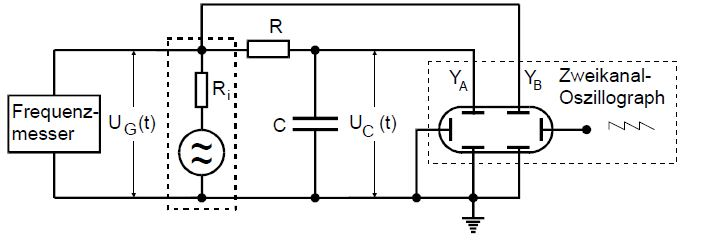
\includegraphics[height=5cm]{RC4.JPG}
  \caption{Messschaltung zur Bestimmung der Phasenverschiebung.}
  \cite{skript}
  \label{fig:RC4}
\end{figure}
Auf dem $Y_{B}$ Eingang der Oszilloskops wird die Kondensatorspannung $U_{C}$
und auf dem $Y_{A}$ Eingang die Generatorspannung $U_{G}$ aufgetragen.
Wenn die Phasenverschiebung größer als Null ist, ergibt sich ein Schirmbild wie in
Abbildung \ref{fig:phase}.
\begin{figure}[H]
  \centering
  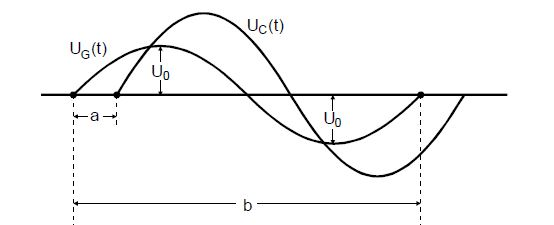
\includegraphics[height=5cm]{phase.JPG}
  \caption{Beipsielhafte Darstellung der Phasenverschiebung der Kondensator- und der Generatorspannung.}
  \cite{skript}
  \label{fig:phase}
\end{figure}
An diesem Schirmbild wird mit Hilfe der Curser-Funktion der Abstand der Nullduchgänge $a$
und die Schwingungsdauer $b$ gemessen. DiePhasenverschiebung kann aus $a$ und $b$ über
diese Formeln berechnet werden:
\begin{align}
  \phi &= \frac{a}{b}\cdot 360 \\
  \phi &= \frac{a}{b}\cdot 2\pi
\end{align}

Um zu zeigen, dass ein RC-Kreis bestimmte Spannungen integrieren kann, wird die
Schaltung aus Abbildung \ref{fig:RC4} verwendet. Die Frequenz der Generatorspannung
wird konstant gehalten und nacheinander wird eine Rechteck-, Sinus- und Dreieckspannung
auf den RC-Kreis gegeben. Das Oszilloskop wird so eingestellt, dass die
angelegte Spannung und die integrierte Spannung eingezeig wird. Von diesem
Schirmbild wird ein Thermodruck angefertigt.
